%%%%%%%%%%%%%%%%%%%%%%%%%%%%%%%%%%%%%%%%%%%%%%%%%%%%%
%
%  Template
%  Beamer Presentation by Chris Bourke
%
%%%%%%%%%%%%%%%%%%%%%%%%%%%%%%%%%%%%%%%%%%%%%%%%%%%%%%%%%%%%%%%%%%%%%%%

\documentclass[]{beamer}
%\documentclass[handout]{beamer}

\geometry{papersize={16cm,9cm}}

% For handout version:
%\usetheme[hideothersubsections,slidenumbers]{UNLTheme}
\usetheme[hideothersubsections]{UNLTheme}
\usepackage{amssymb}
\input{StandardCommands}
\usepackage[linesnumbered,ruled,vlined]{algorithm2e}
\SetKwComment{Comment}{//}{}
\DontPrintSemicolon
\SetKwSty{textsc} %
%\SetAlFnt{\scriptsize} %
\SetKwInOut{Input}{Input} %
\SetKwInOut{Output}{Output} %
%\setalcapskip{1em} % changed to
\SetAlCapSkip{1em}
\setlength{\algomargin}{2em} %
%\Setvlineskip{0em} % changed to:
\SetVlineSkip{0em}

\usepackage{tikz}
\usetikzlibrary{fadings}
\usetikzlibrary{shapes.geometric,shapes.symbols}
\usetikzlibrary{calc,shapes.multipart,chains,arrows}
\usetikzlibrary{arrows.meta,calc,shapes.multipart,chains,arrows}
%\usetikzlibrary{calc,shapes.multipart,chains,arrows}
%%\usetikzlibrary{backgrounds}
\usetikzlibrary{backgrounds}
\usetikzlibrary{decorations.pathreplacing}
\usetikzlibrary{decorations.pathmorphing}
\tikzset{onslide/.code args={<#1>#2}{%
  \only<#1>{\pgfkeysalso{#2}} % \pgfkeysalso doesn't change the path
}}
\tikzset{temporal/.code args={<#1>#2#3#4}{%
  \temporal<#1>{\pgfkeysalso{#2}}{\pgfkeysalso{#3}}{\pgfkeysalso{#4}} % \pgfkeysalso doesn't change the path
}}

\tikzset{
    fading speed/.code={
        \pgfmathtruncatemacro\tikz@startshading{50-(100-#1)*0.25}
        \pgfmathtruncatemacro\tikz@endshading{50+(100-#1)*0.25}
        \pgfdeclareverticalshading[%
            tikz@axis@top,tikz@axis@middle,tikz@axis@bottom%
        ]{axis#1}{100bp}{%
            color(0bp)=(tikz@axis@bottom);
            color(\tikz@startshading)=(tikz@axis@bottom);
            color(50bp)=(tikz@axis@middle);
            color(\tikz@endshading)=(tikz@axis@top);
            color(100bp)=(tikz@axis@top)
        }
        \tikzset{shading=axis#1}
    }
}

\usepackage{multirow}
\usepackage{multicol}

\definecolor{steelblue}{rgb}{0.2745,0.5098,0.7059}
\hypersetup{
    colorlinks = true,
    urlcolor = {steelblue},
    linkbordercolor = {white}
}

\definecolor{mintedBackground}{rgb}{0.95,0.95,0.95}
\definecolor{mintedInlineBackground}{rgb}{.90,.90,1}

%\usepackage{newfloat}
\usepackage{minted}
\setminted{mathescape,
               linenos,
               autogobble,
               frame=none,
               fontsize=\small,
               framesep=2mm,
               framerule=0.4pt,
               %label=foo,
               xleftmargin=2em,
               xrightmargin=0em,
               startinline=true,  %PHP only, allow it to omit the PHP Tags *** with this option, variables using dollar sign in comments are treated as latex math
               numbersep=10pt, %gap between line numbers and start of line
               style=default, %syntax highlighting style, default is "default"
               			    %gallery: http://help.farbox.com/pygments.html
			    	    %list available: pygmentize -L styles
               bgcolor=mintedBackground} %prevents breaking across pages
               
\setmintedinline{bgcolor={mintedInlineBackground}}
\setminted[text]{bgcolor={},linenos=false,autogobble,xleftmargin=1em}

\tikzstyle{decision} = [diamond, draw, fill=yellow!20, 
    text width=6em, text badly centered, node distance=5cm, inner sep=0pt]
\tikzstyle{block} = [rectangle, draw, fill=blue!20, 
    text width=5em, text centered, node distance=5cm, minimum height=4em]
\tikzstyle{action} = [rectangle, draw, fill=green!20, 
    text width=5em, text centered, rounded corners, node distance=5cm, minimum height=4em]
\tikzstyle{line} = [draw, -latex']

\title[~]{Computer Science I}
\subtitle{Functions \& Pointers}
\author[~]{Dr.\ Chris Bourke\\ \email{cbourke@cse.unl.edu}} %
\date{~}

\begin{document}

\begin{frame}
  \titlepage
\end{frame}

\setbeamertemplate{section in toc}{\inserttocsectionnumber.~\inserttocsection}
\setbeamercolor{section in toc}{fg=black}
%\setbeamertemplate{subsection in toc}{~} %\inserttocsubsection\\}

\begin{frame}
  \frametitle{Outline}
%{\footnotesize
%\begin{NoHyper}
%  \tableofcontents[hideallsubsections]
%\end{NoHyper}
%}

\setbeamercolor{enumerate item}{bg=white,fg=black}
\setbeamercolor{item}{bg=white,fg=black}
\setbeamercolor{item projected}{bg=white,fg=black}
\setbeamercolor{enumerate subitem}{fg=red!80!black}
\setbeamertemplate{enumerate items}[default]
\begin{enumerate}
  \item Introduction
    %motivation: top down problem solving, procedural abstraction, etc.
    %declaration, prototypes
    %definition
    %using
  \item Modularity
    %separation into header/source
    %compilation
    %
  \item Pitfalls \& Other Issues
    %keyword: void
    %function overloading
    % return statement: lack caues problems
    % failure to use #include
    %failure to have a prototype? or a prototype mismatch: misspell one of them.
  \item How Functions Work
    %call stack
    %include scope discussion
    %swap example
  \item Pointers
  \item Passing By Reference
\end{enumerate}

\end{frame}

\section{Introduction}

\begin{frame}
    \frametitle{}
    \framesubtitle{}
    
    \begin{center}
    {\Huge Part I: Introduction}\\
    {\Large ~}
    \end{center}

\end{frame}


\begin{frame}
    \frametitle{Functions}
    \framesubtitle{}

\begin{itemize}[<+->]
  \item A function produces an \emph{output} when given an \emph{input} or \emph{inputs}
  \item In math:
    $$f(x) = x^2$$
    $$g(x, y) = 2x + 3y$$
  \item ``Outputs'':
    $$f(3) = 9$$
    $$g(2, 4) = 16$$
  \item It can only ever produce at most \emph{one} output
  \item It may take any number of inputs (including none!)
  \item Functions in code are similar and use familiar ``syntax''
\end{itemize}    

\end{frame}

\begin{frame}[fragile]
    \frametitle{Functions in Code}
    \framesubtitle{}

\begin{itemize}[<+->]
  \item In code, a \emph{function} is a reusable unit of code that 
  may take input(s) and may produce an output
  \item Familiar functions: \mintinline{c}{main()}, \mintinline{c}{printf()},  \mintinline{c}{sqrt()}
\end{itemize}
\end{frame}

\begin{frame}[fragile]
    \frametitle{Functions in Code}
    \framesubtitle{}

\begin{minted}{c}
int main(int argc, char **argv) {

  double x = 2.0;
  double y = sqrt(x);
  
  return 0;
}
\end{minted}
\vskip-.5cm
\begin{itemize}[<+(1)->]
  \item You \emph{call} or \emph{invoke} a function
  \item Functions can be called inside other functions
  \item Function $A$ (``calling function'') calls function $B$ 
  \item A function may ``return'' a value to the calling function 
\end{itemize}    

\end{frame}

\begin{frame}
    \frametitle{Motivation}
    \framesubtitle{}

\begin{itemize}[<+->]
  \item Functions facilitate \emph{code reuse}
    %you don't have to cut-n-paste the same block of code over and over
  \item Procedural abstraction: designing and using functions allows
  you to abstract the details of how a block of code or algorithm works
  %us to ignore the minute details of how a certain block of code or algorithm works
  \item Functions \emph{encapsulate} functionality into reusable, abstract code blocks
  \item Example: how does \mintinline{c}{sqrt()} work?
\end{itemize}    

\end{frame}

\begin{frame}
    \frametitle{Usefulness}
    \framesubtitle{}

\begin{itemize}[<+->]
  \item Standard libraries and external libraries are full of useful functions
  \item Well tested, well designed, efficient and optimized
  \item Functions are fundamental to top-down design
  \item Problem solving: first question you ask is ``is this problem already solved?''
  %that is, does a function already exist to solve my problem?
\end{itemize}    

\end{frame}


\subsection{Declaring}

\begin{frame}[fragile]
    \frametitle{Functions in C}
    \framesubtitle{}

\begin{itemize}[<+->]
  \item Functions must be declared before they can be used
  \item Declare a function using a \emph{prototype} that specifies the
  function's \emph{signature}
  \item Signature:
  \begin{itemize}
    \item Name of the function (\emph{identifier})
    \item A list of its \emph{parameters} or \emph{arguments}; 
    both the \emph{number} and \emph{type}
    \item The function's \emph{return} type: the type of data the function returns
  \end{itemize}
\end{itemize}    

\end{frame}

\begin{frame}[fragile]
    \frametitle{Prototype Example}
    \framesubtitle{}

\begin{minted}[fontsize=\footnotesize]{c}
/**
 *  This function computes the Euclidean distance between
 *  the two points defined by (x1, y1) and (x2, y2)
 */
double euclideanDistance(double x1, double y1, double x2, double y2);
\end{minted}

Syntax and style:
\begin{itemize}[<+->]
  \item Documented using doc-style comments (DRY)
  %vertical stars
  %always place with prototypes
  %DRY
  \item Return type
  \item Identifier: use \mintinline{c}{lowerCamelCasing}
  \item Comma delimited list of parameters and their type
  \item Prototype ends with a semicolon and has no function \emph{body}
\end{itemize}

\end{frame}

\begin{frame}[fragile]
    \frametitle{Definition Example}
    \framesubtitle{}
    
\begin{minted}[fontsize=\footnotesize]{c}
double euclideanDistance(double x1, double y1, double x2, double y2) {

  double temp = sqrt( (x1 - x2) * (x1 - x2) + (y1 - y2) * (y1 - y2) );
  return temp;
}
\end{minted}

\begin{itemize}[<+->]
  \item Signature is repeated but a function \emph{body} is included
  %curly brackets
  \item The \mintinline{c}{temp} variable is a \emph{local} variable
  \item Parameter variables are also \emph{local}
  \item Observe: functions call functions
%After the function is done executing, they no longer exist and are out of scope
%In general, you can declare as many local variables as you want
%In addition, the parameters are treated as local variables

  \item Demonstration
   %write the distance in a full program; emphasize the different variables
   % note the usage: prototype is all that is necessary to use it   
   % temp variable is not in scope, etc.
   % refactor to not use the temp variable
   % demonstrate that a lack of a return leads to undefined behavior
\end{itemize}
\end{frame}


\section{Modularity}

\begin{frame}
    \frametitle{}
    \framesubtitle{}
    
    \begin{center}
    {\Huge Part II: Modularity}\\
    {\Large Writing modular code, creating libraries}
    \end{center}

\end{frame}

\begin{frame}[fragile]
    \frametitle{Modularity}
    \framesubtitle{}
    
\begin{itemize}[<+->]
  \item Modularity refers to the degree to which a system's components 
    can be separated and recombined or reused
  \item In software, this means separating functionality (functions) into
    independent interchangeable modules or ``libraries''
  \item Separation allows you to organize very complex programs
    with thousands or millions of LOCs
  \item Programs only ``include'' the functionality they actually need
\end{itemize}  
  
\end{frame}

\begin{frame}[fragile]
    \frametitle{Modularity in C}
    \framesubtitle{}
    
\begin{itemize}[<+->]
  \item In C, libraries are separated out into different files
  \item Prototypes are placed in a \emph{header} file (ends with \mintinline{text}{.h})
  \item Definitions are placed in a \emph{source} file (ends with \mintinline{text}{.c})
  \item \mintinline{c}{stdio.h}, \mintinline{c}{math.h}
  \item You can then \mintinline{c}{#include} your own libraries!
\end{itemize}

\end{frame}

\begin{frame}[fragile]
    \frametitle{Demonstration}
    \framesubtitle{}
    
\begin{itemize}[<+->]
  \item Separate our distance functionality into:
  \begin{itemize}
    \item Header: \mintinline{text}{distance.h}
    \item Source: \mintinline{text}{distance.c}
    \item Use the same base file name
  \end{itemize}
  \item Include the header file in our main: for \emph{user defined libraries} we generally use \mintinline{c}{#include "distance.h"}
  \item Compile separate modules:
  \begin{itemize}
    \item Compile our distance library:\\    
    \mintinline{text}{gcc -c distance.c}\\
    produces an \emph{object} file, \mintinline{text}{distance.o}
    \item Compile the entire program together including the library files:\\
    \mintinline{text}{gcc distance.o distanceDriver.c}\\
  \end{itemize}    
  \item Add additional distance-related functionality
  %TODO: expand distance library to include manhattan (L1) and air distance
\end{itemize}

\end{frame}


\section{Pitfalls \& Other Issues}

\begin{frame}
    \frametitle{}
    \framesubtitle{}
    
    \begin{center}
    {\Huge Part III: Pitfalls \& Other Issues}\\
    {\Large ~}
    \end{center}

\end{frame}

\subsection{Keyword: void}


\begin{frame}[fragile]
    \frametitle{Void functions}
    \framesubtitle{}

\begin{itemize}[<+->]
  \item Functions are not required to return a value
  \item Functions that do not return a value are called \mintinline{c}{void} functions
  \item Keyword \mintinline{c}{void} is used as the return type
  \item Example: \mintinline{c}{void swap(int a, int b);}
  \item Return statement should still be included: \mintinline{c}{return;}
  \item Functions are not required to take inputs
  \item Functions that do not have any inputs are no-arg functions
  \item Example: \mintinline{c}{int foo(void);}
  \item Better practice to omit \mintinline{c}{void}: \\
  \mintinline{c}{int foo();}
\end{itemize}

\end{frame}

\subsection{Function Overloading}

\begin{frame}[fragile]
  \frametitle{Function Overloading}
  \framesubtitle{}

\begin{itemize}[<+->]
  \item Some languages support \emph{Function Overloading}
  \item \emph{Function Overloading}: multiple functions may share 
  the same identifier (name) as long as they differ in the number or
  type of parameters
  \item C does \emph{not} support function overloading
  \item Consequence: functions that do the same thing but with different
  types all need unique names
  \item Example: \mintinline{c}{abs(int)}, \mintinline{c}{fabs(double)}, 
  \mintinline{c}{labs(long)}
  \item Must take care when naming functions so as not to \emph{pollute the namespace}
\end{itemize}

\end{frame}
    
\subsection{Pitfalls}

\begin{frame}[fragile]
  \frametitle{Missing Return Statements}
  \framesubtitle{}

\begin{itemize}[<+->]
  \item Common mistake: forgetting to include the \mintinline{c}{return} statement
  \item Omission is still syntactically correct; but will not give the intended results
  %arcane rules take over for what the function ends up returning
  \item Can be easily avoided using the \mintinline{text}{-Wall} flag
  \item Demonstration
\end{itemize}

\end{frame}

\begin{frame}[fragile]
  \frametitle{Common Compilation Failures}
  \framesubtitle{}

\begin{itemize}[<+->]
  \item Must use \mintinline{c}{#include} and you \emph{only} ever include header files
  %include both failure in driver file and in source file
  %show that without the prototype, you can give an incorrect number of arguments
  \item Prototypes should always be included
  \item Prototype and definition signatures \emph{must} match
  %otherwise they define different functions.
  \item Demonstration
\end{itemize}

\end{frame}


\section{How Functions Work}

\begin{frame}
    \frametitle{}
    \framesubtitle{}
    
    \begin{center}
    {\Huge Part IV: How Functions Work}\\
    {\Large ~}
    \end{center}

\end{frame}

\begin{frame}[fragile]
  \frametitle{How Functions Work}
  \framesubtitle{}

\begin{minipage}[t]{0.6\linewidth}
\begin{itemize}[<+->]
  \item Programs have a \emph{program stack}
  \item Stack: Last-In First-Out (LIFO)
  \item Push: add something to the top
  \item Pop: remove something from the top
\end{itemize}
\end{minipage}
\begin{minipage}[t]{0.30\linewidth}
\onslide<2->{

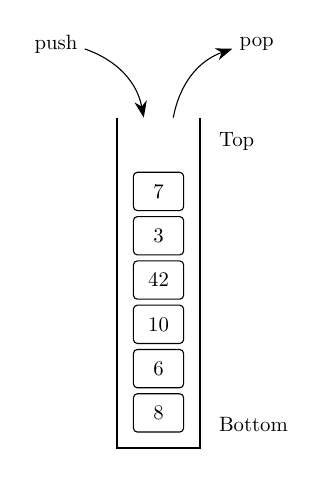
\begin{tikzpicture}[scale=.75,transform shape,
    list/.style={draw,inner sep=6pt,
    rounded corners=.5mm,minimum width=.85cm},
    node distance=.75cm]
  
  \node[list] (A) {8};
  \node[list,above of=A] (B) {6};
  \node[list,above of=B] (C) {10};
  \node[list,above of=C] (D) {42};
  \node[list,above of=D] (E) {3};
  \node[list,above of=E] (F) {7};
  
  \draw[-,thick] (-.70,5) -- (-.70,-.6) -- (.70,-.6) -- (.70, 5);
  
  \node[right] at (.90,-.2) {Bottom};
  \node[right] at (.90,4.6) {Top};
  
  \node[left] (PUSH) at (-1.25,6.25) {push};
  \node[right] (POP) at (1.25,6.25) {pop};
  
  \draw[-{Stealth[scale=1.25]}] (PUSH) to [bend left] (-.25,5);
  \draw[{Stealth[scale=1.25]}-] (POP) to [bend right] (.25,5);
  
\end{tikzpicture}
}
\end{minipage}

\end{frame}

\begin{frame}[fragile]
  \frametitle{Program Stack}
  \framesubtitle{}

\begin{itemize}[<+->]
  \item At the start of a program, a program call stack is created
  \item At the bottom, the program code is loaded
  \item Global variables and static content are added
  \item As functions are called, a new stack frame is created
  \item Each frame contains: parameters, local variables, etc.
  \item When a function returns, the frame is popped from the top of the call stack
  \item Data and variables in each frame is distinct and separate
\end{itemize}

\end{frame}

\begin{frame}[fragile]
  \frametitle{Program Stack}
  \framesubtitle{}


\begin{minted}{c}
double sum(double a, double b) {
  double x = a + b;
  return x;
}

double average(double a, double b) {
  double y = sum(a, b) / 2.0;
  return y;
}

int main(int argc, char **argv) {
  double a = 10.0, b = 16.0;
  double ave = average(a, b);
  printf("average = %f\n", ave);
  return 0;
}
\end{minted}

\end{frame}

\begin{frame}[plain,fragile]
  \frametitle{Program Stack}
  \framesubtitle{}
  
\begin{minipage}[c]{0.50\linewidth}
\begin{tikzpicture}[auto,scale=0.45,transform shape,every node/.style={text centered, text width=5.5cm}]

\node [above left] (bottom) at (0,0) {Bottom of the stack (high memory)};
\node [below left] (top) at (0,15.5) {Top of the stack (low memory)};

\draw (6,18.5) -- (6, 15.5);
\draw[path fading=north] (0,15.5) -- (0, 18.5);
\node [above] (unused) at (3, 16) {Unused stack space};

\draw[fill=blue!10!white] (0, 0) rectangle (6,2);
\node [above] (pc) at (3,0) {Program Code};

\draw[fill=yellow!10!white] (0, 2) rectangle (6,3.5);
\node [above] (globals) at (3,2) {Global Variables \\ Static Content};

\draw[fill=green!30!white] (0, 3.5) rectangle (6,7.5);
\node [above] (main) at (3,3.5) {arguments \mintinline{c}{argc, argv}};
\draw[dashed] (0, 5) -- (6, 5);
\node [above] (mainvar) at (3,5) {return address, value (\mintinline{c}{0})};
\draw[dashed] (0, 6) -- (6, 6);
\node [above] (mainvar2) at (3,6) {local variables \mintinline{c}{a, b, ave}};
\draw [decorate,decoration={brace,amplitude=10pt,mirror},xshift=4pt,yshift=0pt] (6, 3.5) -- (6, 6.5+1) node [align=left,black,midway,xshift=6.5cm]  {\texttt{main()} stack frame};


\draw[fill=green!20!white] (0, 3.5+4) rectangle (6,7.5+4);
\node [above] (main) at (3,3.5+4) {arguments \mintinline{c}{a, b}};
\draw[dashed] (0, 5+4) -- (6, 5+4);
\node [above] (mainvar) at (3,5+4) {return address, value (\mintinline{c}{13.0})};
\draw[dashed] (0, 6+4) -- (6, 6+4);
\node [above] (mainvar2) at (3,6+4) {local variables \mintinline{c}{y}};
\draw [decorate,decoration={brace,amplitude=10pt,mirror},xshift=4pt,yshift=0pt] (6, 3.5+4) -- (6, 7.5+4) node [align=left,black,midway,xshift=6.5cm]  {\texttt{average()} stack frame};


\draw[fill=green!10!white] (0, 3.5+8) rectangle (6,7.5+8);
\node [above] (main) at (3,3.5+8) {arguments \mintinline{c}{a, b}};
\draw[dashed] (0, 5+8) -- (6, 5+8);
\node [above] (mainvar) at (3,5+8) {return address, value (\mintinline{c}{26.0})};
\draw[dashed] (0, 6+8) -- (6, 6+8);
\node [above] (mainvar2) at (3,6+8) {local variables \mintinline{c}{x}};
\draw [decorate,decoration={brace,amplitude=10pt,mirror},xshift=4pt,yshift=0pt] (6, 3.6+8) -- (6, 7.6+8) node [align=left,black,midway,xshift=6.5cm]  {\texttt{sum()} stack frame};
\end{tikzpicture}

\end{minipage}~~~~~~\begin{minipage}[c]{0.35\linewidth}
\begin{itemize}[<+->]
  \item Stack orientation
  \item Each function has its own stack frame
  \item Parameters/arguments are \emph{passed by value} to the function
  \item The values stored in the variables are copied into variables in a new
  stack frame
  \item As functions return, stack frames are removed
  \item Live demonstration
\end{itemize}
\end{minipage}


\end{frame}

\begin{frame}[fragile]
  \frametitle{Demonstration}
  \framesubtitle{}
  
Consider the following code that attempts to swap two values:
\begin{minted}{c}
void swap(int a, int b) {
  int temp = a;
  a = b;
  b = temp;
  return;
}
\end{minted}

%swap demo

\end{frame}

\section{Pointers}

\begin{frame}
    \frametitle{}
    \framesubtitle{}
    
    \begin{center}
    {\Huge Part V: Pointers}\\
    {\Large ~}
    \end{center}

\end{frame}

\begin{frame}[fragile]
  \frametitle{Memory}
  \framesubtitle{}

\begin{itemize}[<+->]
  \item Every piece of data in a computer is stored in memory
  \item Memory has both an \emph{address} and \emph{contents}
\end{itemize}
\onslide<2->{\tiny
\begin{center}
\begin{tabular}{|l|l|}
\multicolumn{1}{c}{Address} & \multicolumn{1}{c}{Contents} \\
\hline
\texttt{0x7fff58310b87} & \texttt{0x01} \\
\hline
\texttt{0x7fff58310b86} & \texttt{0x32} \\
\hline
\texttt{0x7fff58310b85} & \texttt{0x7c} \\
\hline
\texttt{0x7fff58310b84} & \texttt{0xff} \\
\hline
\texttt{0x7fff58310b83} & \texttt{~} \\
\texttt{0x7fff58310b82} & \texttt{~} \\
\texttt{0x7fff58310b81} & \texttt{~} \\
\texttt{0x7fff58310b80} & \texttt{~} \\
\texttt{0x7fff58310b7f} & \texttt{~} \\
\texttt{0x7fff58310b7e} & \texttt{~} \\
\texttt{0x7fff58310b7d} & \texttt{~} \\
\texttt{0x7fff58310b7c} & \texttt{3.14159265359} \\
\hline
\texttt{0x7fff58310b7b} & \texttt{~} \\
\texttt{0x7fff58310b7a} & \texttt{~} \\
\texttt{0x7fff58310b79} & \texttt{~} \\
\texttt{0x7fff58310b78} & \texttt{32,321,231} \\
\hline
\texttt{0x7fff58310b77} & \texttt{~} \\
\texttt{0x7fff58310b76} & \texttt{~} \\
\texttt{0x7fff58310b75} & \texttt{~} \\
\texttt{0x7fff58310b74} & \texttt{1,458,321} \\
\hline
\multicolumn{1}{c}{$\vdots$} & \multicolumn{1}{c}{$\vdots$} \\
\end{tabular}
\end{center}
}

\end{frame}

\begin{frame}[fragile]
  \frametitle{Pointers}
  \framesubtitle{}

\begin{itemize}[<+->]
  \item In C, you can access memory \emph{contents} with variables
  \item You can access memory \emph{addresses} with \emph{pointers}
  \item A pointer is a memory reference that ``points'' to some memory address
  \item Syntax:
\begin{minted}{c}
//regular variable:
int a = 10;

//an integer pointer variable:
int *ptrToA;
\end{minted}
\end{itemize}
  
\end{frame}

\begin{frame}[fragile]
  \frametitle{Pointers}
  \framesubtitle{}

\mintinline{c}{int *ptrToA;}
\begin{itemize}[<+->]
  \item \mintinline{c}{ptrToA} is a pointer variable that can point to a memory
  location that stores an integer
  \item An \emph{uninitialized pointer} may point to anything:
  \begin{itemize}
    \item Non-existant memory location
    \item Memory location that doesn't belong to us
    \item \mintinline{text}{0xDEADBEEF}
  \end{itemize}
  \item Best practice to initialize pointers
  \item The \mintinline{c}{NULL} pointer is a special pointer that indicates ``nothing''
  \item Initialization:\\
  \mintinline{c}{int *ptrToA = NULL;}
\end{itemize}
  
\end{frame}

\begin{frame}[fragile]
  \frametitle{Pointers}
  \framesubtitle{Other Types}

\begin{itemize}[<+->]
  \item Pointer variables can be created for any type of variable.
\begin{minted}{c}
int *ptrToA = NULL;
double *ptrToB = NULL;
char *ptrToC = NULL;
\end{minted}

  \item You can also test for nullity:
\begin{minted}{c}
if(ptrToA == NULL) {
  printf("Error: ptrA points to nothing!\n");
}
\end{minted}
  \item Null pointer check
\end{itemize}

\end{frame}


\begin{frame}[fragile]
  \frametitle{Using Pointers}
  \framesubtitle{Referencing Operator}

\begin{itemize}[<+->]
  \item Need to be able to make a pointer \emph{point} to something
  \item Usual assignment operator works, but \emph{both sides must match}
  \item Referencing operator, \mintinline{c}{&} gives the \emph{memory address} of a regular variable
  \item[~]
\begin{minted}{c}
int a = 42;
int *ptrToA = NULL;

//make ptrToA point to a:
ptrToA = &a;
\end{minted}
  \item[~]
\begin{minted}{c}
double b = 10.5;
double *ptrToB = NULL;
ptrToB = &b;
\end{minted}
\end{itemize}
    
\end{frame}

\begin{frame}[fragile]
  \frametitle{Pitfalls}
  \framesubtitle{}

\begin{itemize}[<+->]
  \item Types of pointer variables and what they point to \emph{need to match}:
\begin{minted}{c}
int a = 42;
double *dblPtr = NULL;
dblPtr = &a; //WRONG
\end{minted}
  \item Pointers \emph{must be assigned a valid memory address}
\begin{minted}{c}
int a = 42;
int *ptrToA = NULL;
ptrToA = a;  //WRONG!!
ptrToA = 10; //SO WRONG!!
\end{minted}

\end{itemize}

\end{frame}


\begin{frame}[fragile]
  \frametitle{Using Pointers}
  \framesubtitle{Dereferencing Operator}

\begin{itemize}[<+->]
  \item Once a pointer points to something, we need a way to get to the memory \emph{contents}  
  \item The \emph{dereferencing operator}, \mintinline{c}{*} ``changes'' a pointer into
  a regular variable
  \item[~]
\begin{minted}{c}
int a = 42;
int *ptrToA = &a;

int b = *ptrToA + 10;
\end{minted}
  \item You can also \emph{change} the contents
\begin{minted}{c}
*ptrToA = 43;
\end{minted}
\end{itemize}
    
\end{frame}


\begin{frame}[fragile]
  \frametitle{Summary}
  \framesubtitle{}

\begin{itemize}[<+->]
  \item Pointer declaration:\\
  \mintinline{c}{int *ptr = NULL;}
  \item Pointer initialization and referencing operator:\\
  \mintinline{c}{ptr = &a;}
  \item Dereferencing operator:
  \mintinline{c}{*ptr = 43;}
  \item Demonstration
  \item Why pointers?  
  \item So we can \emph{pass variables by reference}!!
\end{itemize}

\end{frame}



\section{Pass By Reference}

\begin{frame}
    \frametitle{}
    \framesubtitle{}
    
    \begin{center}
    {\Huge Part VI: Pass By Reference}\\
    {\Large ~}
    \end{center}

\end{frame}

\begin{frame}[fragile]
  \frametitle{Pass By Reference}
  \framesubtitle{}

\begin{itemize}[<+->]
  \item Recall our swap function:
\begin{minted}{c}
void swap(int a, int b) {
  int temp = a;
  a = b;
  b = temp;
  return;
}
\end{minted}
  \item Failed because \mintinline{c}{a} and \mintinline{c}{b} were passed
  by value
  \item Values were copied to separate local parameter variables
  \item Using pointers, we can pass \emph{references} to the variables instead
  
\end{itemize}

\end{frame}

\begin{frame}[fragile]
  \frametitle{Pass By Reference}
  \framesubtitle{}
  
\begin{itemize}[<+->]
  \item Parameters become pointer variables instead:
  \item[~]
\begin{minted}{c}
void swap(int *a, int *b) {
  int temp = *a;
  *a = *b;
  *b = temp;
  return;
}
\end{minted}
  \item You've actually seen this before!
  \item \mintinline{c}{scanf("%d", &x);}
  \item Demonstration
\end{itemize}

\end{frame}

\begin{frame}[fragile]
  \frametitle{Pass By Reference}
  \framesubtitle{Summary}

\begin{itemize}[<+->]
  \item Passing by reference means that \emph{pointers} to variables are passed
  instead of copies
  \item Functions can make changes that are \emph{visible} to the calling function
  \item Consequences: 
  \begin{itemize}
    \item Functions can have \emph{side effects}
    \item Functions can ``return'' multiple values via pass-by-reference variables
  \end{itemize}
\end{itemize}
  
\end{frame}


\begin{frame}[fragile]
  \frametitle{Pass By Reference}
  \framesubtitle{Summary}

Demonstration:
\begin{enumerate}
  \item Modify one of our distance functions to utilize pass-by-reference
  \item Implement a new function to calculate a line graph:
    $$y = mx + b$$
  Given $(x_1, y_1), (x_2, y_2)$, compute:
  $$m = \frac{\Delta y}{\Delta x} = \frac{y_2-y_1}{x_2-x_1}$$
  $$b = y_1 - m x_1$$
\end{enumerate}

\end{frame}


\end{document} 
